\section{\name Framework} \label{sec:tgm_frame}

In this section, we present the formal foundations of \name. We unify continuous- and discrete-time formulations into a common representation, define graph discretization as a principled mapping from continuous events to snapshots, and introduce the hook formalism, a modular abstraction for composing graph operations. Together, these elements inform the software design in Section~\ref{sec:software}.

% \subsection{\name Temporal Graph Formulation} \label{sec:tg_formulation}

\textbf{\name Temporal Graph Formulation.}
First, we introduce the notation and treatment of temporal graphs in \name. On temporal graphs, events are the fundamental unit for representing the network’s evolution~\citep{DBLP:journals/jmlr/KazemiGJKSFP20}. To capture changes in graph structure and features, we distinguish between event types:

\begin{definition}[Node and Edge Events]
An edge event $(t, s, d, \vec{x}_{edge})$ is an interaction between two nodes $s$ and $d$ at time $t$ where $\vec{x}_{edge}\in \mathbb{R}^{d_{edge}}$ is the associated edge feature vector. A node event $(t, s, \vec{x}_{node})$ represents the arrival of new features $\vec{x}_{node} \in \mathbb{R}^{d_{node}}$ at node $s$ and timestamp $t$. 
\end{definition}

\definition[Temporal Graph] \label{def:tg} A temporal graph is a sequence of time-ordered events: $\mathcal{G} = \{e_0, ..., e_T\}$. Each event $e_i$ can be an edge event or a node event. Also, $\mathcal{G}$ can be associated with a static node feature matrix $\mat{X} \in \mathbb{R}^{n \times d_{static}}$ where $n$ is the number of unique nodes in $\mathcal{G}$. For any time interval $\mathcal{T} \subset \mathbb{R}^+$, the temporal sub-graph $\mathcal{G}|_{\mathcal{T}}$ contains all events in $\mathcal{G}$ intersecting $\mathcal{T}$. 


\begin{figure*}[t]
  \centering
% \includegraphics[width=0.8\linewidth]{iclr_2026/artifacts/time_ops.pdf}
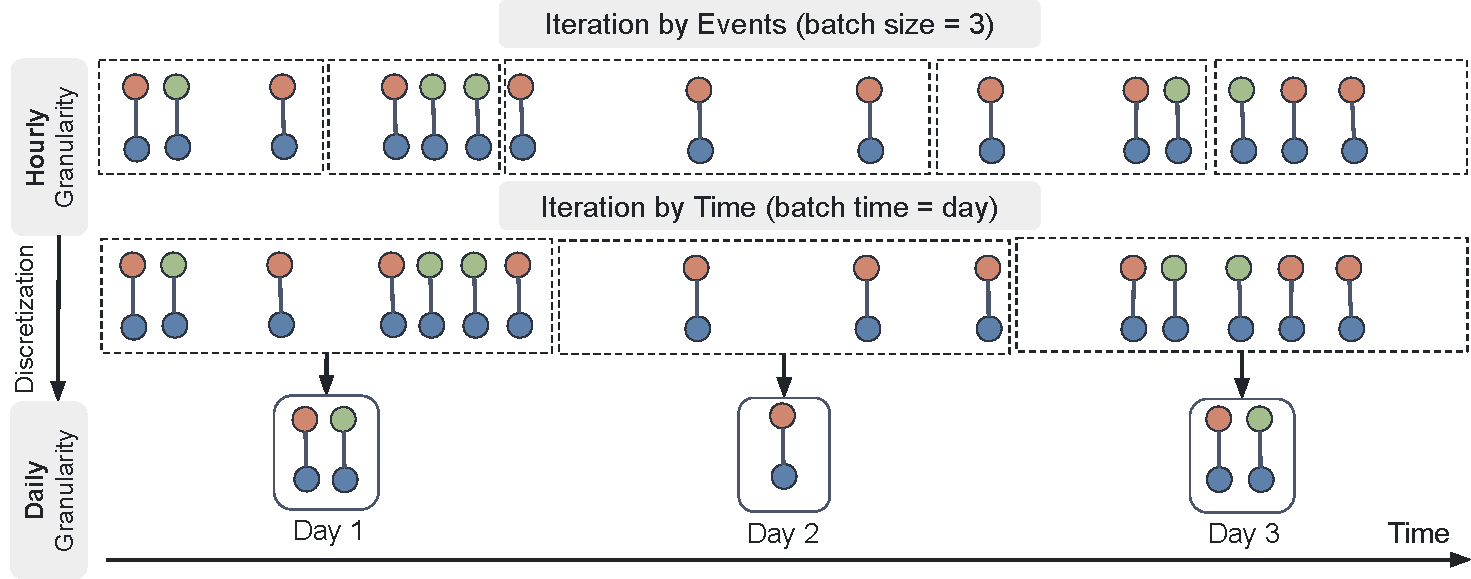
\includegraphics[width=\linewidth]{iclr_2026/artifacts/tgm_time.pdf}
  \caption{\name supports iteration by events and time. Discretization maps fine-grained timestamps (e.g., hourly) to coarser timestamps (e.g., daily), aggregating duplicated edges in the process.}
  \label{fig:time_ops}
\end{figure*}


\textbf{Representing Continuous-Time and Discrete-Time Graphs.} In \name, we represent temporal graphs as event sequences without distinguishing between CTDG and DTDG formulations. We argue that any temporal graph admits a native time granularity $\tau$: the coarsest unit of time (e.g., seconds) that still discriminates between all event timestamps. If real-world time is unavailable (e.g., due to privacy), \name employs a special event-ordered granularity $\tau_{\text{event}}$, preserving only the relative order of events but lacks correspondence to a real-world time granularity, thus $\tau_{\text{event}}$ is excluded from any time operations. Lastly, note that time granularities can be compared: $\hat{\tau} \leq \tau \iff \tau \textit{ is coarser than } \hat{\tau}$. This view unifies CTDG and DTDG as alternative ways of iterating over the same event stream:


\definition[CTDG: Event-based iteration] A CTDG is often expressed as a stream of events~\citep{DBLP:journals/jmlr/KazemiGJKSFP20,DBLP:conf/nips/HuangPDFHRLBRR23, tgn, DBLP:conf/kdd/YouDL22}. In \name, iterating a CTDG corresponds to using the event-ordered granularity $\tau_{\text{event}}$. Each batch contains a fixed number of events, independent of real-world time.

\definition[DTDG: Time-based iteration] A DTDG is often expressed as a sequence of static graph snapshots sampled at regularly-spaced time intervals, i.e. as $\{\mat{G}_0, \mat{G}_1, ..., \}$, where $\mat{G}_i = \{\mat{V}_i, \mat{E}_i\}$ is a static graph at snapshot $i$~\citep{utg}. 
In \name, we achieve this by iterating with a time granularity $\hat{\tau}$ that is coarser than the native graph granularity. Iterating by time produces batches $\mathcal{G}|_{[t_0, t_i]}, \mathcal{G}|_{[t_i, t_{i + 1}]}, \cdots$ where $|t_i - t_0| = |t_{i+1} - t_i| = \hat{\tau}$. 

\textbf{Discretizing Temporal Graphs.} For snapshot-based models, it is often useful to process the graph at a coarser granularity than the native $\tau$ (e.g., daily instead of second-wise). Discretization converts the underlying network to this coarser timeline by collapsing duplicate edges within each time interval:

\definition[Time Granularity Discretization.] Let $\mathcal{G}$ be a temporal graph with native time granularity $\tau$. For any $\hat{\tau} \geq \tau$, the discretization operator:
\begin{align}
    \mathcal{\psi}_{r}: (\mathcal{G}, \tau) \mapsto (\hat{\mathcal{G}}, \hat{\tau})
\end{align}
maps $\mathcal{G}$ to coarser granularity $\hat{\tau}$, groups events into equivalence classes induced by $\hat{\tau}$ and applies a reduction operator $r$ to each class. The resulting graph 
$\hat{\mathcal{G}}$ contains one representative event per class. Figure~\ref{fig:time_ops} illustrates these time operations in \name.

\textbf{\name Learning Tasks}
The common goal in TG is to forecast the structure or property of the graph in the future. \name supports ML on all levels of the graph, namely link, node and graph tasks:
\begin{itemize}[leftmargin=*, noitemsep, topsep=0.2pt]
\item \textbf{Dynamic Link Property Prediction.} Given the temporal sub-graph $\mathcal{G}|_{[t_0, t_i]}$, predict some property (or existence) of a link between a node pair $(s,d)$ at a future timestamp $t$ where $t > t_i$.  
\item \textbf{Dynamic Node Property Prediction.} Given the temporal sub-graph $\mathcal{G}|_{[t_0, t_i]}$, predict some property of a node $s$ at a future timestamp $t$ where $t > t_i$.  
\item \textbf{Dynamic Graph Property Prediction.} Given the temporal sub-graph $\mathcal{G}|_{[t_0, t_i]}$, predict some property of $\mathcal{G}|_{[t', t'']}$ over a future time interval $[t', t'']$ where $t_i < t'\leq t''$.
\end{itemize}





% \begin{table}[t]
% \centering
% \renewcommand{\arraystretch}{1}
% \small
% \begin{tabular}{l|ccccc}
% \toprule
% \textbf{Hook Type} 
% & \multicolumn{2}{c}{\textbf{Neighbor Sampling}} 
% & \textbf{Evaluation} 
% & \multicolumn{1}{c}{\textbf{Device Ops}} 
% & \multicolumn{1}{c}{\textbf{Analytics}} \\
% & Recency
% & Uniform
% & TGB Eval
% & GPU Transfer
% & DOS Estimate \\
% \midrule
% $\mathcal{R}$ (Requires) & $\{\text{negatives}\}$ & $\{\text{negatives}\}$ & $\emptyset$ & $\emptyset$ & $\emptyset$ \\
% $\mathcal{P}$ (Produces)  & $\{\text{neighbors}\}$ & $\{\text{neighbors}\}$ & $\{\text{negatives}\}$ & $\emptyset$ & $\{\text{DOS}\}$ \\
% \midrule
% \end{tabular}

% \caption{Examples of common temporal graph operations represented as hooks, and their attributes.}
% \label{tab:hooks}
% \end{table}

% \subsection{\name Hooks and Recipes}
% \label{sec:hooks}
\textbf{\name Hooks and Recipes.} We formalize a TGL workflow as a composition of transformations called hooks. Each hook specifies a typed contract on batch attributes, and recipes are valid precisely when their signatures compose. 

\begin{definition}[Materialized Batch] Let $G|_{\mathcal{T}}$ be a temporal subgraph. We denote by $B|_{\mathcal{T}, \mathcal{A}}$ the materialized batch associated with a set of properties $\mathcal{A}$. Intuitively, $\mathcal{A}$ captures the attributes that enrich the slice of data, typically tensors required by a model (e.g. neighborhood information in message-passing architectures). 
\end{definition}


\begin{definition}[Hook] A hook $\phi_{\mathcal{R}, \mathcal{P}}$ is a transformation on a materialized batch:
\begin{align}
    \phi_{\mathcal{R}, \mathcal{P}}: \mathcal{B}|_{\mathcal{T}, \mathcal{A}} \mapsto \mathcal{B}|_{\mathcal{T}, \mathcal{A} \cup \mathcal{P}}
\end{align}
which declares a contract based on the attributes required on the input $\mathcal{R} \subset \mathcal{A}$, and the attributes produced $\mathcal{P}$, so that the batch transformed by $\phi$ has attributes $\mathcal{A} \cup \mathcal{P}$. Table \ref{tab:hooks} illustrates several common temporal graph operations expressed as hooks using the notation introduced here.
\end{definition}

The real power of hooks is unlocked by composing their transformations to express complete temporal graph workflows. The notion of a hook recipe formalizes this.


\begin{definition}[Hook Recipe] A set of hooks $\{\phi^1_{\mathcal{R}_1, \mathcal{P}_1}, ..., \phi^k_{\mathcal{R}_k, \mathcal{P}_k}\}$ induces an ordering given by their dependencies:
\begin{align}
    \phi^i \to  \phi^j \iff \mathcal{P}_i\cap \mathcal{R}_j \neq \emptyset
\end{align}

We call this a hook recipe if this dependency graph is acyclic and every required is satisfied, i.e. $\forall j, \mathcal{R}_j \subset \bigcup_{i < j} \mathcal{P}_i$. Thus, any hook recipe admits a valid ordering by topological sort.
With this framework, exploring new research is simpler as complex workflows can be expressed with minimal boilerplate. Figure~\ref{fig:recipe} illustrates how ML and analytics pipelines are represented as recipes in \name.
\end{definition}



\begin{table}[t]
\centering
\renewcommand{\arraystretch}{1}
\caption{Examples of common temporal graph operations represented as hooks, and their attributes.}
\label{tab:hooks}
\resizebox{0.9\linewidth}{!}{%
\begin{tabular}{l|ccccc}
\toprule
\textbf{Hook Type} 
& \multicolumn{2}{c}{\textbf{Neighbor Sampling}} 
& \textbf{Evaluation} 
& \multicolumn{1}{c}{\textbf{Device Ops.}} 
& \multicolumn{1}{c}{\textbf{Analytics}} \\
& Recency
& Uniform
& TGB Eval
& GPU Transfer
& DOS Estimate \\
\midrule
$\mathcal{R}$ (Requires) & $\{\text{negatives}\}$ & $\{\text{negatives}\}$ & $\emptyset$ & $\emptyset$ & $\emptyset$ \\
$\mathcal{P}$ (Produces)  & $\{\text{neighbors}\}$ & $\{\text{neighbors}\}$ & $\{\text{negatives}\}$ & $\emptyset$ & $\{\text{DOS}\}$ \\
\midrule
\end{tabular}
}
\end{table}

\begin{figure*}[t]
  \centering
  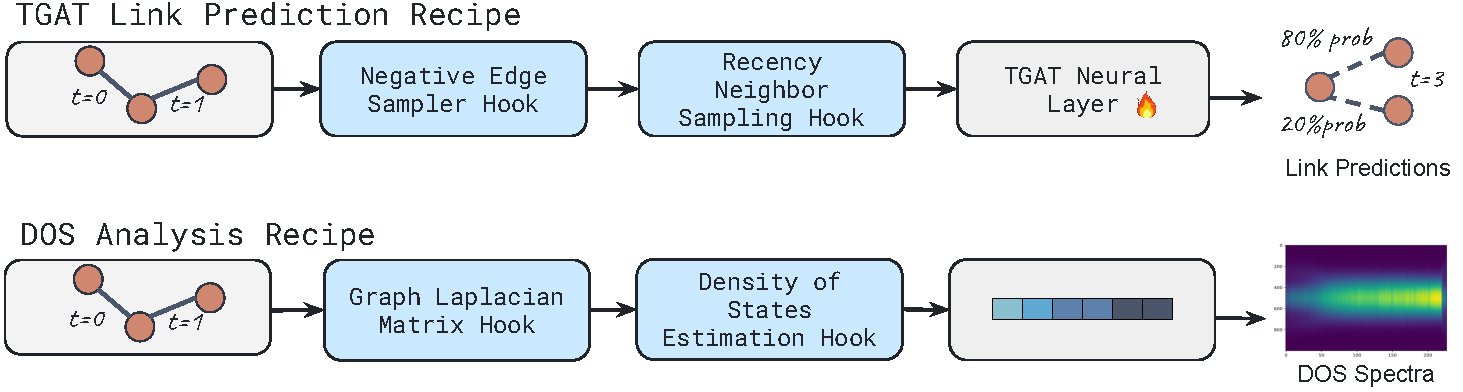
\includegraphics[width=0.85\linewidth]{iclr_2026/artifacts/tgm_recipe.pdf}
  \caption{Example recipes in \name: TGAT link prediction and Density of States Analysis. \name provides a unified ecosystem supporting both representation learning and temporal graph analytics. The constituent hooks are modular, enabling reuse across different workflows within the community.}
  \label{fig:recipe}
\end{figure*}
